\chapter{Dateien}
\label{chp:Files}
\epigraph{
	The only superstition I have is that I must start a new book on the same day that I finish the last one, even if it's just a few notes in a file. I dread not having work in progress.
}{Terry Pratchett}

Ausgaben auf dem Bildschirm sind temporär -- Daten auf der Festplatte sind für immer\footnote{Eigentlich nur für die nächsten Jahre, abhängig vom Speichermedium. In jedem Fall aber lang genug...}. Hier werden wir uns der Aufgabe stellen, Daten vom Arbeitsspeicher auf dauerhafte Speichermedien\footnote{In der Regel auf die Festplatte} zu schreiben und von dort wieder in den Arbeitsspeicher zu lesen.

\section{Binäre und Text-Dateien}
Zuerst wollen wir aber einige Gedanken zur internen Darstellung von Daten aufwenden.

Wie Sie wissen, sind im Speicher alle Daten \emph{binär} abgelegt, \ie als Pattern von Einsen und Nullen. Je nach Kontext werden diese Pattern auf unterschiedliche Weise interpretiert.

Eine Folge von Bits $b_i$ kann zum Beispiel nach dieser Formel als Ganzzahl\footnote{Eine ähnliche, jedoch schwerer zu verstehende Formel existiert auch für Fließkommazahlen. Interessierte KursteilnehmerInnen können sich über die Norm IEEE 754 informieren (siehe hierzu beispielsweise \url{https://de.wikipedia.org/wiki/IEEE_754}). Für hier reicht es vollkommen, zu verstehen, dass Kommazahlen und Ganzzahlen nach unterschiedlichen Regeln in den Speicher geschrieben werden} $n$ interpretiert werden:
\begin{equation*}
	n = \sum_{i} 2^n \; b_i
\end{equation*}

Dasselbe Pattern kann aber auch für ein Schriftzeichen stehen. In diesem Fall wird mittels einer Tabelle übersetzt. Jedes Schriftzeichen hat eine Nummer, die leicht als Binärzahl darstellbar ist und in dieser Form das Zeichen im Arbeitsspeicher repräsentiert. Die ersten 128 Schriftzeichen sind in Abbildung \ref{fig:ASCII} gezeigt\footnote{ASCII -- American Standard Code for Information Interchange -- stellt einen der ältesten Standards dar, der in der Westlichen Welt lange Zeit genutzt wurde. Darauf aufbauend existieren ANSI, Unicode in diversen Implementationen, ... -- \emph{It's a mess.} Allen diesen Standards ist gemeinsam, dass einem Schriftzeichen ein \emph{Codepoint} zugeordnet ist, dass es also mit einer Ganzzahl identifiziert wird.}.

\begin{figure}
\begin{center}
	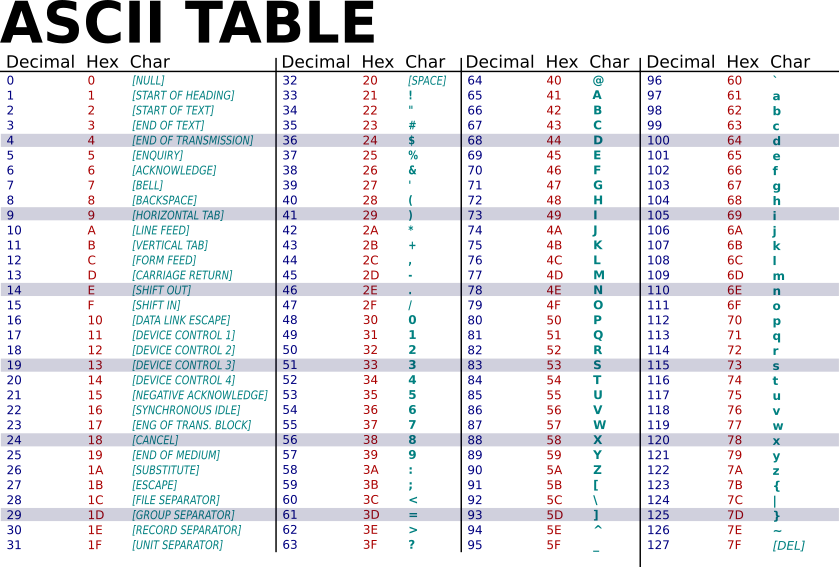
\includegraphics[width=.8\linewidth]{./gfx/ASCII_table}
	\caption[
		ASCII-Tabelle: Lookup-Tabelle zur Interpretation von Zahlen als Schriftzeichen
	]{
		ASCII-Tabelle: Lookup-Tabelle zur Interpretation von Zahlen als Schriftzeichen\\
		Quelle: \url{https://en.wikipedia.org/wiki/File:ASCII-Table-wide.svg}
	}
	\label{fig:ASCII}
\end{center}
\end{figure}

Wenn Sie sich diese Tabelle durchsehen, wird Ihnen auffallen, dass darin auch wieder Ziffern vorkommen. Das bedeutet, dass eine Zahl sowohl durch ihr Bitmuster dargestellt werden kann, als auch durch die Bitmuster ihrer Textdarstellung. Die Zahl \inPy{42} hat etwa das Bitmuster \texttt{00101010}. Als \emph{Text} \inPy{"42"} finden wir dagegen die Schriftzeichen \inPy{"4"} und \inPy{"2"} mit ASCII-Codes 52 und 50 und daher der das Bitmuster \texttt{00110110 00110100}. Genauso kann auch das Bitmuster \texttt{00101010} als das \emph{Schriftzeichen} mit der Nummer 42 gelesen werden, also als \inPy{"*"}.

Bisher mussten wir uns mit der Frage der Interpretation von Daten kaum beschäftigen, da jeder Ausdruck in Python einen zugeordneten \emph{Datentypen} hat; die Regeln zur Interpretation werden also \enquote{kostenlos} mitgeliefert. In Dateien dagegen können wir dagegen nur rohe Daten speichern. Als ProgrammiererInnen müssen wir uns also überlegen, wie und von wem diese Daten interpretiert werden sollen.

Wir unterscheiden im Wesentlichen zwischen \emph{Binärdaten} und \emph{Textdaten}. Binärdaten werden so auf die Festplatte geschrieben, wie sie auch im Speicher vorliegen, und auch so von dort gelesen. Man könnte sagen, Binärdaten seien die Muttersprache der Computer. Textdaten dagegen werden zuerst so übersetzt, dass sie ein menschlicher Leser leicht übersetzen kann.

In einem Beispiel: Sie haben im Speicher die \inPy{int}-Zahl \inPy{42}. Im Binärmodus wird daher das zugehörige Bitmuster \texttt{00101010} auf die Festplatte geschrieben. Öffnen wir diese Datei mit einem \emph{Text}editor, sehen wir das Zeichen \texttt{*}.\\
Wird dieselbe Zahl \inPy{42} dagegen im Textmodus geschrieben, so übersetzt Python diese zuerst in den \emph{Text} \inPy{"42"}, und schreibt dann diesen auf die Festplatte. Wir finden also das Bitmuster \texttt{00110110 00110100}. In einem Texteditor lesen wir auch wieder \texttt{42}.

Python erledigt all dieses Übersetzen für uns im Hintergrund. Wir als ProgrammiererInnen müssen aber zumindest vorgeben, ob eine Datei im Binärmodus oder im Textmodus gelesen/geschrieben werden soll.

\section{Einfacher Dateizugriff}
Python stellt \enquote{einfache Hausmittel} zur Arbeit mit Dateien zur Verfügung. Darauf aufbauend existieren weitere Module, die uns die Arbeit erleichtern, für die wir aber auch die \enquote{Hausmittel} im Prinzip verstanden haben müssen. 

\subsection{Dateien Öffnen und Schließen}
Um mit Dateien umzugehen, brauchen wir zunächst ein \emph{Handle auf die Datei}. Das ist eine Variable, in der alle nötigen Hintergrund-Informationen (Speicherort, Dateigröße, Netzwerkdatei oder lokale Datei, ...) zusammengefasst sind. Es handelt sich also um eine Klasseninstanz, deren Eigenschaften wir hier oberflächlich kennen lernen wollen. Stellen Sie sich das Handle tatsächlich als einen \enquote{Griff} vor, der an eine Datei angebracht wird: mit diesem Griff können Sie die Datei anpacken und darin Operationen (Lesen, Schreiben, Analysieren) durchführen.

Wir erhalten ein solches Handle über den Befehl \inPy{open}:
\begin{codebox}[Syntax: \texttt{open}]
\begin{minted}{python3}
handle = open(Dateiname, Modus)
\end{minted}
\end{codebox}

Wie zu erwarten ist \texttt{Dateiname} ein String, der den Namen der Datei enthält, die geöffnet werden soll. Je nach Betriebssystem wird Groß- und Kleinschreibung unterschieden\footnote{Unter Windows wird nicht unterschieden. Linux und Mac dagegen erkennen \texttt{file} und \texttt{File} als unterschiedliche Dateien an.}. Die Datei wird im \emph{aktuellen Arbeitsverzeichnis} erwartet, \ie in dem Ordner, von dem aus Python auch gestartet wurde. Üblicherweise ist das derselbe Pfad, in dem auch Ihre Script-Datei liegt. Sollen Dateien in anderen Ordnern betrachtet werden, können aber auch \emph{absolute} und \emph{relative} Pfadangaben gemacht werden:

Absolute Pfadangaben enthalten die volle Information, wo im Dateisystem eine Datei abgelegt ist. Sie beginnt mit einem Betriebssystem-spezifischen Symbol für die \emph{Wurzel} des Dateisystems (\enquote{root}), und durch \emph{Forward Slashes /}\footnote{Unter Windows sind auch \emph{Backslashes} \textbackslash erlaubt und z.\;T. noch üblich. Dies bereitet aber oft Probleme mit Escape-Sequenzen und sollte daher vermieden werden} voneinander abgetrennte Ordnernamen. Unter Windows ist dieses Wurzel-Zeichen der \emph{Laufwerks-Buchstabe} gefolgt von einem Doppelpunkt. Ein gültiger Dateiname mit absoluter Pfadangabe unter Windows könnte also lauten:
\begin{center}
	\texttt{C:/User/some\_folder/myFile.txt}
\end{center}
Linux und Mac verwalten Laufwerke anders; die Wurzel des Dateisystems ist daher durch einen einfachen Forward Slash gekennzeichnet:
\begin{center}
	\texttt{/home/user/some\_folder/myFile.txt}
\end{center}

Relative Pfadangaben gehen vom aktuellen Arbeitsverzeichnis aus. Von diesem Startpunkt aus wird die Orderstruktur navigiert. Dass eine Pfadangabe relativ sein soll, wird erklärt, indem man als erstes Zeichen einen Punkt angibt.

Beispiel: Ihre Code-Datei liegt unter \texttt{/home/user/Codes/}. Die Datei, die Sie öffnen wollen, befindet sich in \texttt{/home/user/Codes/files}. In dem Fall können Sie auf diese Datei zugreifen, indem Sie als \inPy{Dateiname} angeben:
\begin{center}
	\texttt{./files/myFile.txt}
\end{center}
Dies gilt so gleichermaßen für Windows als auch für Linux und Mac.

Ist die Datei in einem \emph{Überordner}, so kann dies mit \emph{zwei Punkten} angezeigt werden. Wir können auch mehrere ebenen zurück gehen, indem wir Punkte und Slashes aneinander reihen: \texttt{../../} bezeichnet den Ordner \emph{zwei Ebenen} über dem Arbeitsverzeichnis. Weiter können wir diese Schreibweise auch mit relativen Pfadangaben kombinieren. Stellen wir uns wieder vor, das aktuelle Arbeitsverzeichnis wäre \texttt{/home/user/Codes/}. Die Datei, die Sie öffnen wollen, efindet sich nun aber im Order \texttt{/home/user/files}. In diesem Fall geben Sie an:
\begin{center}
	\texttt{../files/myFile.txt}
\end{center}


Unter \emph{Modus} verstehen wir, für welche Art Zugriff die Datei geöffnet werden soll. Wollen wir aus der Datei Lesen oder Schreiben? Soll der Zugriff im Text- oder Binärmodus stattfinden? Der Modus wird durch einen String beschrieben. Die wichtigsten Modi finden Sie in Tabelle \ref{tab:FileModes}:

\begin{center}
\rowcolors{1}{white}{tabhighlight}
\begin{tabular}{c|cp{.6\linewidth}}
	\toprule
	\textbf{String}	& \textbf{Bedeutung}				& \textbf{Kommentar} \tabcrlf
	\texttt{r}				& Lesen -- Textmodus				& Dateicursor am Anfang der Datei.\newline Neuen Dateien werden \emph{nicht} angelegt.\\
	\texttt{rb}			& Lesen -- Binärmodus			& Dateicursor am Anfang der Datei.\newline Neuen Dateien werden \emph{nicht} angelegt.\\
	\texttt{w}				& Schreiben -- Textmodus		& Dateicursor am Anfang der Datei.\newline Neuen Dateien werden angelegt, alte Dateien überschrieben.\\
	\texttt{wb}			& Schreiben -- Binärmodus	& Dateicursor am Anfang der Datei.\newline Neuen Dateien werden angelegt, alte Dateien überschrieben.\\
	\texttt{x}				& Schreiben -- Textmodus		& Dateicursor am Anfang der Datei.\newline Neuen Dateien werden angelegt, alte Dateien \emph{nicht} überschrieben.\\
	\texttt{xb}			& Schreiben -- Binärmodus	& Dateicursor am Anfang der Datei.\newline Neuen Dateien werden angelegt, alte Dateien \emph{nicht} überschrieben.\\
	\texttt{a}				& Anhängen -- Textmodus		& Dateicursor am \emph{Ende} der Datei. Neuen Dateien werden angelegt, alte Dateien \emph{nicht} überschrieben.\\
	\texttt{ab}			& Anhängen -- Binärmodus		& Dateicursor am \emph{Ende} der Datei. Neuen Dateien werden angelegt, alte Dateien \emph{nicht} überschrieben. \\
	\bottomrule
\end{tabular}
\captionof{table}{Dateimodi in python3}
\label{tab:FileModes}
\end{center}

\begin{hintbox}[Relative Pfadangaben bevorzugen]
Absolute Pfadangaben sind von Natur aus unflexibel. Wenn Sie Ihr Programm an Kollegen verschicken, wird es vermutlich nicht mehr funktionieren. Bevorzugen Sie daher relative Pfadangaben, und konzipieren Sie nach Möglichkeit Ihre Programme so, dass notwendige Dateien in \emph{Unterordnern} liegen.
\end{hintbox}

Jede Datei, die geöffnet wurde, sollte auch wieder geschlossen werden. Dies geschieht mit der Methode \inPy{close}:
\begin{codebox}[Syntax: \texttt{open}]
\begin{minted}{python3}
handle.close()
\end{minted}
\end{codebox}

Ob eine Datei noch geöffnet ist, können wir mit dem Attribut \inPy{closed} in Erfahrung bringen: \inPy{handle.closed} ist entweder \inPy{True} oder \inPy{False}.

\subsection{Dateien Schreiben}
\subsubsection{Textmodus}
Sobald eine Datei in einem Text-Schreibmodus geöffnet wurde (\texttt{w},  \texttt{x} oder \texttt{a}), und solange sie noch nicht wieder geschlossen wurde, können wir mit der Methode \inPy{write} Text in eine Datei schreiben. Die Syntax ist denkbar einfach:

\begin{codebox}[Syntax: \texttt{write}]
\begin{minted}{python3}
handle.write(Text)
\end{minted}
\end{codebox}

Dabei ist \inPy{Text} ein beliebiger Ausdruck, der zu einem String ausgewertet werden kann.

\begin{codebox}[Beispiel: Text-Dateien Schreiben]
\begin{minted}[linenos]{python3}
handle = open("output.txt", "w")    # Text/Schreibmodus

handle.write("Some text\n")
handle.write("another line " * 2 + "\n")
handle.write( str(handle) )

handle.close()
\end{minted}
\end{codebox}

\begin{cmdbox}[Dateinhalt von \texttt{output.txt}]
\begin{minted}{text}
Some text
another line another line 
<_io.TextIOWrapper name='output.txt' mode='w' encoding='UTF-8'>
\end{minted}
\end{cmdbox}

Beachten Sie, dass, anders als bei \inPy{print} Zeilenumbrüche \emph{nicht} automatisch angehängt werden. Diese müssen explizit als \inPy{"\n"} teil des zu schreibenden Strings sein.

Im obigen Beispiel wird der \emph{Rückgabewert} der Methode ignoriert. \inPy{write} gibt die Zahl der in die Datei geschriebenen Bytes zurück. Dieses Feature wird selten gebraucht, kann aber unter Umständen nützlich sein.

Öffnen wir nach Zeile dieselbe Datei \texttt{output.txt} nochmals in den Modi \texttt{w}, \texttt{wb}, \texttt{x} oder \texttt{xb}, so wird der Dateiinhalt sofort gelöscht. Bei den Modi \texttt{a} und \texttt{ab} dagegen bleibt der alte Inhalt bestehen; neu geschriebener Text wird an das Ende der Datei angehängt.

\subsubsection{Binärmodus}
Schreiben im Binärmodus funktioniert prinzipiell genauso, wie wir es vom Textmodus schon kennen: Öffnen mit \inPy{open} in einem geeigneten Modus (\texttt{wb},  \texttt{xb} oder \texttt{ab}), Schreiben mit \inPy{handle.write(data)} und Schließen mit \inPy{handle.close()}. An das Objekt \inPy{data} muss \emph{eindeutig} in eine Byte-Sequenz übersetzt werden können. (Eingangs wurde gesagt, dass \eg der \inPy{int}-Wert \inPy{42} in das Bitpattern \texttt{00101010} übersetzt wird; gleichermaßen ist aber auch das Bitpattern \texttt{00000000 00101010} denkbar, und eine beliebige andere Zahl führender Nullen. Die Gründe hierfür sind leider etwas technisch, und können an dieser Stelle nicht erschöpfend erklärt werden).

Eine Klasse von Objekten, das eine solche absolut unmissverständliche Darstellung haben, sind Instanzen der Klasse \inPy{bytes}. Diese können beispielsweise aus \inPy{list}s erstellt werden, wenn deren einzelne Elemente nur Werte zwischen \inPy{0} und \inPy{255} annehmen.

\begin{codebox}[Beispiel: Binär-Dateien Schreiben]
\begin{minted}[linenos]{python3}
handle = open("output.dat", "wb")    # Binär/Schreibmodus

data = bytes([65, 66, 67])
handle.write( data )

handle.close()
\end{minted}
\end{codebox}

\begin{cmdbox}[Dateinhalt von \texttt{output.dat}]
\begin{minted}{text}
ABC
\end{minted}
\end{cmdbox}


\subsection{Dateien Lesen}
Das Lesen aus Dateien gestaltet sich ähnlich einfach wie das Schreiben: nachdem die Datei in einem geeigneten Modus geöffnet wurde (\texttt{r} oder \texttt{rb}) kann mit den Methoden \inPy{read} und \inPy{readline} gearbeitet werden.

Beim Lesen können wir uns vorstellen, dass in der Datei ein \enquote{Cursor} platziert wird. Zu Beginn ist dieser ganz am Anfang der Datei. Mit jedem Lese-Befehl wandert dieser Cursor dann vorwärts. Gelesen wird immer jeweils von der aktuellen Cursorposition.

Die Methode \inPy{read} im einfachsten Fall \emph{die gesamte Datei} in den Arbeitsspeicher:
\begin{codebox}[Syntax: \texttt{read}]
\begin{minted}{python3}
StringVariable = handle.read()
\end{minted}
\end{codebox}

Optional kann auch ein \inPy{int}-Parameter \inPy{size} mit übergeben werden. Dieser gibt eine Maximalmenge an Daten an, die aus der geöffneten Datei \inPy{handle} gelesen werden dürfen. 
\begin{codebox}[Syntax: \texttt{read} (erweitert)]
\begin{minted}{python3}
StringVariable = handle.read(size)
\end{minted}
\end{codebox}
Dabei bezeichnet \inPy{size} die Zahl der Bytes, die maximal gelesen werden dürfen.

Die online-Dokumentation (\url{https://docs.python.org/3/tutorial/inputoutput.html}) kommentiert hierzu lakonisch:
\begin{center}
	\emph{It’s your problem if the file is twice as large as your machine’s memory.}
\end{center}

Beispiel: Wir wollen die im vorigen Abschnitt vorbereitete Datei \texttt{output.txt} zurück in den Arbeitsspeicher lesen. Dies erreichen wir mit dem folgenden Code:
\begin{codebox}[Beispiel: Text-Dateien Lesen]
\begin{minted}[linenos]{python3}
handle = open("output.txt", "r")    # Text/Lesemodus

firstWord = handle.read(4)
rest      = handle.read()

handle.close()

print(firstWord)
print(rest)
\end{minted}
\end{codebox}

\begin{cmdbox}[Ausgabe: Text-Dateien Lesen]
\begin{minted}{text}
Some
 text
another line another line 
<_io.TextIOWrapper name='output.txt' mode='w' encoding='UTF-8'>
\end{minted}
\end{cmdbox}

Der Dateiinhalt wird als String in den Speicher geladen. Soll dieser wieder als Zahl behandelt werden, so muss der String mit den entsprechenden Funktionen (\inPy{int()}, \inPy{float()}, ...) umgewandelt werden.

Wird \enquote{nach dem Ende der Datei} versucht, weiter zu lesen, so ist das Ergebnis einfach ein leerer String.

Textdateien sollen besonders häufig Zeile für Zeile bearbeitet werden. Zu diesem Zweck existiert die Methode \inPy{readline}:
\begin{codebox}[Syntax: \texttt{readline}]
\begin{minted}{python3}
StringVariable = handle.readline(size)
\end{minted}
\end{codebox}
\inPy{readline} liest von der aktuellen Cursorposition bis zum nächsten Zeilenumbruch. Wieder begrenzt der Parameter \inPy{size} die Datenmenge, die maximal gelesen wird. Wird dieser ausgelassen oder wird hier ein negativer Wert übergeben, so liest Python \emph{die gesamte Zeile}.

Verwandt mit der Methode \inPy{readline} ist die Methode \inPy{readlines}: Diese liest \emph{die gesamte Datei}, zerlegt sie dabei aber bereits an den Zeilenumbrüchen, und packt die Teilde der Datei in eine \inPy{list}:

\begin{codebox}[Beispiel: \texttt{readlines}]
\begin{minted}[linenos]{python3}
handle = open("output.txt", "r")    # Text/Lesemodus

lines = handle.readlines()

handle.close()

for line in lines :
    print(line)
\end{minted}
\end{codebox}

Beachten Sie, dass die Zeilenumbrüche selbst beim Lesen nicht entfernt werden. Entsprechend sehen wir bei diesem Beispiel zusätzliche, leere Zeilen:

\begin{cmdbox}[Ausgabe: \texttt{readlines}]
\begin{minted}{text}
Some text

another line another line 

<_io.TextIOWrapper name='output.txt' mode='w' encoding='UTF-8'>
\end{minted}
\end{cmdbox}


\subsection{Dateien und Blockstrukturen}
Im Kontext von Dateien können Sie das Schlüsselwort \inPy{with .. as} benutzen. Damit wird eine neue Umgebung (Einrückungsebene) geschaffen, innerhalb derer eine Datei geöffnet ist. Sehen Sie also \inPy{with} als eine Kurzform an, die automatisch eine geöffnete Datei schließt, wenn die Einrückungsebene von \inPy{with} geschlossen wird.

\begin{codebox}[Syntax: \texttt{with .. as}]
\begin{minted}[linenos]{python3}
with open(Dateiname, Modus) as Handle :
    Datei_Anweisungen
\end{minted}
\end{codebox}

Das oben gezeigte \emph{Beispiel: Text-Dateien Schreiben} lässt sich also auch so schreiben:
\begin{codebox}[Beispiel: Text-Dateien Schreiben]
\begin{minted}[linenos]{python3}
with open("output.txt", "w") as handle :
    handle.write("Some text\n")
    handle.write("another line " * 2 + "\n")
    handle.write( str(handle) )
\end{minted}
\end{codebox}

Wie schon zuvor wird die Datei \texttt{\enquote{output}} im Schreibmodus geöffnet und mit drei Zeilen gefüllt. Mit dem Ende von Zeile 4 wird die Datei automatisch geschlossen.

\begin{hintbox}[\texttt{with}-Blocks für eigene Klassen: \texttt{\_\_enter\_\_} und \texttt{\_\_exit\_\_}]
Wie Sie sich denken können, sind Handles nur Instanzen einer Klasse, nämlich \inPy{_io.TextIOWrapper}. Die gezeigten Methoden \inPy{write}, \inPy{read} und \inPy{close} sind im Prinzip nichts anderes, als die Methoden, die Sie im letzten Kapitel bereits kennengelernt haben.

Das Verhalten, das über \inPy{with} erreicht wird, realisiert der Python-Interpreter durch aufruf zweier Dunders erreicht:

Die Methode \inPy{__enter__(self)} wird mit Beginn des \inPy{with}-Blocks aufgerufen. Der Parameter \inPy{self} ist dabei gleich dem Objekt, das hinter \inPy{with} steht. In der Zeile\\
\inPy{with open("output.txt", "w") as handle}\\
erhält \inPy{self} also den Rückgabewert von \inPy{open}. Der Rückgabewert sollte das Objekt \inPy{self} einfach durchreichen.

Die Methode \inPy{__exit__(self, exc_type, exc_value, exc_traceback)} wird aufgerufen, sobald der \inPy{with}-Block verlassen werden soll. Dies kann entweder sein, weil sein Ende erreicht wurde, oder weil im Code des \inPy{with}-Blocks ein Fehler aufgetreten ist. Die Fehlerbeschreibung ist dann in den Variablen \inPy{exc_...} enthalten. Hierauf soll in Kapitel \ref{chp:Exceptions} näher eingegangen werden.
\end{hintbox}

Die weit häufigste Aufgabe im Kontext von Dateien ist, diese Zeile für Zeile zu lesen und mit den geladenen Daten weitere Operationen zu bewerkstelligen (\eg aufsummieren, plotten, ...). Zu diesem Zweck können \inPy{for}-Schleifen verwendet werden:

\begin{codebox}[Syntax: Dateihandles mit \texttt{for}]
\begin{minted}[linenos]{python3}
for Zeile in handle :
    Anweisungen
\end{minted}
\end{codebox}

Diese Syntax enthält also bereits die Mechanik, die Sie sonst mit \inPy{handle.readline} umsetzten würden. Hier wird auch automatisch detektiert, ob das Dateiende bereits erreicht wurde.

Wenn Sie tatsächlich den gesamten Dateiinhalt nach Zeilen aufgetrennt im Speicher brauchen, können Sie das Datei-Handle auch einfach in eine \inPy{list} umwandeln:

\begin{codebox}[Beispiel: Dateihandles als \texttt{list}]
\begin{minted}[linenos]{python3}
with open("output.txt", "r") as handle :
    allLines = list(handle)
    print("Zeile 1:",  allLines[0])
\end{minted}
\end{codebox}

Dies ist vollkommen gleichwertig zu \inPy{allLines = handle.readlines()}

\subsection{Dateicursor Bewegen und Bestimmen}
Manchmal (selten) ist es nötig, die aktuelle Cursorposition in der Datei zu kennen oder zu verändern. Dazu dienen die Methoden \texttt{tell} und \texttt{seek}.

\inPy{handle.tell()} gibt die aktuelle Position des Cursors ab Dateianfang zurück. Mit anderen Worten, der nächste \inPy{read}- oder \inPy{write}-Befehl wirkt auf die Bytes ab Position \inPy{handle.tell()}.

Mit \inPy{seek} kann der Dateicursor verschoben werden. Die hat einen verpflichtenden Parameter \texttt{offset} und einen optionalen Parameter \texttt{from}. Offset gibt an, um wie viele Bytes der Dateicursor gegen einen bestimmten Referenzpunkt verschoben werden soll. Welcher Referenzpunkt das ist, wird über den Parameter \texttt{from} angegeben:
\begin{itemize}
\item Ist \texttt{from == 0} oder wird \texttt{from} ausgelassen, so bezieht sich \texttt{offset} auf den Dateianfang. Mit anderen Worten, \texttt{offset} ist die neue Position des Dateicursors.
\item Ist \texttt{from == 1}, so ist der Referenzpunkt die aktuelle Position. \inPy{handle.seek(-10, 1)} verschiebt also den Dateicursor um 10 Bytes \emph{nach vorne}.
\item Schließlich bedeutet \texttt{from == 2} einen Bezug auf das Dateiende. \inPy{handle.seek(0, 2)} verschiebt also den Dateicursor \emph{an das Dateiende}.
\end{itemize}

\begin{codebox}[Beispiel: Funktion zum Ermitteln der Länge einer Datei]
\begin{minted}[linenos]{python3}
def length_of_file(handle) :
    if handle.closed :
        raise Exception("Datei muss geöffnet sein!")
    
    oldPos = handle.tell()
    
    handle.seek(0, 2)        # an das Dateiende springen
    length = handle.tell()   # Cursorposition Dateiende = Länge!
    
    handle.seek(oldPos)      # Ausgangszustand wiederherstellen
    return length


with open("output.txt", "r") as handle :
    print(handle.name, "ist", length_of_file(handle), "Bytes lang.")
\end{minted}
\end{codebox}



\section{Pickle und JSON}
Die Berechnungen, die Sie in Python umsetzen, können sehr Zeit- und Ressourcen-Aufwändig sein. Wenn dieselben Ausgangsdaten für mehrere Teilprojekte gebraucht werden können, bietet es sich an, diese einmalig auf der Festplatte zu speichern, anstatt sie in jedem Teilprojekt neu zu berechnen. In diesem Fall sind die Daten also nicht für einen menschlichen Betrachter vorgesehen, sondern sollten von einem Computer möglichst effizient geschrieben und wieder entpackt werden können. Die Module \inPy{pickle} (englisch: Gewürzgurke) und JSON (\emph{JavaScript Object Notation} bieten hierzu einige Werkzeuge, die genau diese Aufgaben erledigen.

\subsection{Pickle}
Bei Pickle handelt es sich um ein Python-eigenes Format, das einige spezifische Eigenschaften der Sprache und seines Unterbaus ausnutzt, um sehr verschiedene Objekte bequem für die Archivierung in Dateien vorzubereiten. Leider kann hier nicht auf alle Details eingegangen werden; als Grundsatz können Sie sich jedoch merken:
\begin{center}
	\emph{Wenn Sie es in Python programmiert haben, können Sie es mit Pickle auf der Festplatte abspeichern.}
\end{center}

\begin{warnbox}[Sicherheitslücke Pickle]
Der oben genannte Satz gilt so weit, dass Sie mit Pickle sogar Programmroutinen abspeichern können. Dies erlaubt leider auch, schadhaften Code in Pickle-Archiven unterzubringen. Laden Sie daher nur Archive aus vertrauenswürdigen Quellen (\eg selbst erstellte Archive oder Ergebnisse von ArbeitskollegInnen am selben Projekt). Vertrauen Sie hingegen niemals Archiven, die über das Internet bereitgestellt werden.
\end{warnbox}

Das Archivieren mit Pickle läuft in drei Schritten ab: 
\begin{itemize}
\item Laden des Moduls: \inPy{import pickle}
\item Öffnen einer Datei im Binär-Schreibmodus: \inPy{handle = open(Dateiname, "wb")}
\item Schreiben in eine Datei mit der Methode \texttt{dump}: \inPy{pickle.dump(Objekt, handle)}
\end{itemize}

In ähnlicher Manier kann mit \inPy{Objekt = pickle.load(handle)} ein Objekt aus der Archiv-Datei entpackt werden, und im Anschluss wie eine normale Variable weiter verwendet werden. Unter Objekt ist hierbei tatsächlich eine Variable beliebigen Typs zu verstehen (also \eg \inPy{int}, \inPy{complex}, Klasseninstanzen, Funktionen, ...).

\begin{codebox}[Beispiel: Zahl und Klassenobjekt in Datei zwischenspeichern und wieder laden]
\begin{minted}[linenos]{python3}
import pickle

class Foo :
    def __init__(self) :
        self.bar = 1 + 1j
        
    def __str__(self) :
        return "Foo object"

complexNumber = -0.3 + 4.1j
classObject   = Foo()

with open("archive.pkl", "wb") as handle :
    pickle.dump(complexNumber, handle)
    pickle.dump(classObject  , handle)

with open("archive.pkl", "rb") as handle :
    readComplex     = pickle.load(handle)
    readClassObject = pickle.load(handle)

print(readComplex)
print(readClassObject, readClassObject.bar)
\end{minted}
\end{codebox}

\begin{cmdbox}[Ausgabe: Zahl und Klassenobjekt in Datei zwischenspeichern und wieder laden]
\begin{minted}{text}
(-0.3+4.1j)
Foo object (1+1j)
\end{minted}
\end{cmdbox}

In einer Datei können also beliebig viele Objekte gespeichert werden. Diese Objekte können dann in derselben Reihenfolge zurück gelesen werden, in der sie auch geschrieben wurden.

Der Inhalt der Datei \texttt{archive.pkl} ist nicht für menschliche Betrachter vorgesehen. Je nach Programm, das Sie zum Lesen benutzen, werden Sie eine Kette für Sie sinnloser Zeichen sehen oder auch nur eine Fehlermeldung erhalten.

\begin{hintbox}[Dateinamen und Module]
Sie haben den Befehl \inPy{import} bereits kennengelernt, um Programmkomponenten zu laden, die Sie dann im Anschluss benutzen können. Was dabei geladen wird, ist in der Regel normaler Python-Code. Die Zeile \inPy{import pickle} veranlasst also den Interpreter dazu, die Datei \texttt{pickle.py} zu suchen und die darin definierten Klassen und Methoden bereitzustellen. Diese Datei \texttt{pickle.py} wird dabei \emph{zuerst} im aktuellen Arbeitsverzeichnis gesucht, und dann in einer Reihe von Standard-Ordnern, die bei der Installation von Python festgelegt wurden.

Wenn Sie das obige Beispiel \emph{Beispiel: Zahl und Klassenobjekt in Datei zwischenspeichern und wieder laden} als \texttt{pickle.py} abspeichern, werden Sie daher eine Fehlermeldung erhalten. Achten Sie also darauf, ihre Code-Dateien nicht nach den Modulen zu benennen, die Sie benutzen wollen.
\end{hintbox}

\subsection{JSON}
JSON bezeichnet eine Syntax, mit der verschiedene Datenstrukturen als Text in Dateien abgelegt werden können. Der Fokus liegt hierbei auf Portierbarkeit: JSON-Dateien sollen von möglichst für Programme in möglichst vielen Sprachen verwertbar sein. Dies schränkt die Verwendbarkeit in Python leider leicht ein: nicht jedes beliebige Objekt kann direkt mit JSON archiviert werden. Stattdessen ist es oft nötig, komplexe Datenobjekte (Klasseninstanzen) in kleinere Objekte zu zerlegen (\inPy{list}s, \inPy{dict}s, ...), und diese dann zu schreiben. (Für fortgeschrittene ProgrammiererInnen besteht auch die Möglichkeit, JSON um eigene Encoder/Decoder zu erweitern und so auch komplexere Objekte ohne weitere Vorarbeit in Dateien abzulegen. Darauf kann hier leider nicht eingegangen werden.)

JSON-Dateien sind Text-Dateien, können also von einem menschlichen Betrachter gelesen und verstanden werden. Darin schadhaften Code unterzubringen ist bedeutend schwieriger (wenn auch nicht ganz unmöglich). Das JSON-Format ist also die richtige Wahl für Sie, wenn Sie in Python Daten zu Zwischenergebnissen verarbeiten, die von anderen Programmen gelesen werden sollen, welche nicht in Python geschrieben sind, oder wenn das Lesen der Ergebnisse für einen Menschen ebenfalls möglich sein soll.

Die folgenden Python-Datentypen können in JSON direkt codiert werden:

\begin{minipage}{.49\linewidth}
\begin{itemize}
\item \inPy{int}
\item \inPy{float}
\item \inPy{str}
\item \inPy{bool}
\end{itemize}
\end{minipage}
\begin{minipage}{.49\linewidth}
\begin{itemize}
\item \inPy{list}
\item \inPy{tuple}
\item \inPy{dict}
\item \inPy{None}
\end{itemize}
\end{minipage}

Diese Datentypen können auch ineinander verschachtelt sein, \ie man kann auch ein \inPy{dict} mit mehreren \inPy{list}s ablegen, die ihrerseits wieder komplexere Datenstrukturen aus der oben genannten Liste enthalten.

Der Datentyp \inPy{complex} dagegen wird \emph{nicht} unterstützt. Komplexe Zahlen müssen also entweder in Real- und Imaginärteil zerlegt werden und so als zwei \inPy{float}s gespeichert oder zu einem \inPy{str} umgewandelt werden.

Ähnlich wie bei pickle sind für das Archivieren mit JSON drei Schritte notwendig: 
\begin{itemize}
\item Laden des Moduls: \inPy{import json}
\item Öffnen einer Datei im Text-Schreibmodus: \inPy{handle = open(Dateiname, "w")}
\item Schreiben in eine Datei mit der Methode \texttt{dump}: \inPy{json.dump(Objekt, handle)}
\end{itemize}

Zum Lesen ihres Archivs öffnen Sie die Datei im Text-Lesemodus (\inPy{"r"}), und benutzen die Methode \inPy{json.load}.

Damit die Datei später auch wieder gelesen werden kann, darf nur ein einziges Objekt geschrieben werden. Wollen Sie mehrere Objekte in derselben Datei ablegen, so können Sie diese zu einem \inPy{dict} zusammenfassen.

\begin{codebox}[Beispiel: Archive schreiben und lesen mit JSON]
\begin{minted}[linenos]{python3}
import json

complexNumber = -0.3 + 4.1j

realPart      = complexNumber.real
imaginaryPart = complexNumber.imag

dictionary  = {1 : "one", 2 : "two", 3 : "three"}

with open("archive.json", "w") as handle :
    json.dump(
        {"real" : realPart,
         "imag" : imaginaryPart,
         "dict" : dictionary},
        handle
    )
    
with open("archive.json", "r") as handle :
    jsonObjects = json.load(handle)
    

readComplex = complex(jsonObjects["real"], jsonObjects["imag"])

print(readComplex)
print(jsonObjects["dict"])*
\end{minted}
\end{codebox}

\begin{cmdbox}[Ausgabe: Archive schreiben und lesen mit JSON]
\begin{minted}{text}
(-0.3+4.1j)
{'1': 'one', '2': 'two', '3': 'three'}
\end{minted}
\end{cmdbox}

\begin{cmdbox}[Dateiinhalt: \texttt{archive.json}]
\begin{minted}{text}
{"real": -0.3, "imag": 4.1, "dict": {"1": "one", "2": "two", "3": "three"}}
\end{minted}
\end{cmdbox}

Unter \url{https://www.w3schools.com/python/python_json.asp} finden Sie noch einige weitere Erläuterungen sowie zusätzliche Features, die hier nicht besprochen werden sollen.

\section{CSV-Dateien}
CSV steht für \emph{comma separated values} und ist ein Datenformat, das sich besonders für Tabellen eignet. Wie es der Name suggeriert, werden die einzelnen Spalten der Tabelle durch Trennzeichen voneinander abgesetzt. In der Regel sind diese Trennzeichen Kommata; jedes beliebige andere Zeichen kann jedoch auch als Trennzeichen verwendet werden. CSV-Dateien werden von vielen Programmen als Ausgabeformat unterstützt; unter anderem erlauben es Tabellenkalkulationsprogramme wie Microsoft Excel, Daten im CSV-Format auszugeben.

\begin{tcolorbox}[title=Beispiel CSV-Dateien]
Die folgende Tabelle:

\begin{tabular}{lll}
	Name     & Superkraft                       & Codenummer \\
	Victoria & hat einen Eigenwert              & 80085 \\
	Lea      & verwandelt sich in ein Chamäleon & 1337 \\
	Martina  & ist eigentlich Legolas           & 8453
\end{tabular}

\vspace{6pt}
kann als CSV-Datei abgebildet werden. Das Datei-Abbild könnte dann folgendermaßen aussehen:
\begin{cmdbox}[Datei: \texttt{superheroines.txt}]
\begin{minted}{text}
"Name","Superkraft","Codenummer"
"Victoria","hat einen Eigenwert",80085
"Lea","verwandelt sich in ein Chamäleon",1337
"Martina","ist eigentlich Legolas",8453
\end{minted}
\end{cmdbox}

Wie Sie sehen, werden Texte auch in Anführungszeichen eingerahmt; Zahlen bleiben ohne Sonderzeichen. Während dies eine häufige Wahl bei CSV-Dateien ist, können auch andere Formatierungen gewählt werden.

Im weiteren wollen wir davon ausgehen, dass die gezeigte Datei unter dem Dateinamen \texttt{superheroines.txt} im aktuellen Arbeitsverzeichnis liegt.
\end{tcolorbox}

Das Python-Modul \texttt{csv} erlaubt es, genau solche Date-n strukturiert einzuladen. Zentrales Element ist die Klasse \texttt{csv.reader}, die auf einen bestimmten \emph{Dialekt} von CSV-Formaten eingestellt werden kann (\eg Trennzeichen zwischen Spalten, Anführungszeichen bei Texten, etc.), und die anhand dieser Einstellungen eine Datei in den Arbeitsspeicher liest und in Spalten zerteilt.

Um eine Instanz der Klasse \texttt{csv.reader} zu erhalten, wird ihr Konstruktor aufgerufen. Diesem muss ein Dateihandle im Text-Lesemodus mitgegeben werden. Das Trennzeichen für Spalten über das optionale Schlüsselwort \texttt{delimiter} festgelegt werden:

\begin{codebox}[Beispiel: Datei mit CSV-Reader lesen]
\begin{minted}[linenos]{python3}
import csv
with open("superheroines.txt", "r") as file :
    rdr = csv.reader(file, delimiter=",")
\end{minted}
\end{codebox}

Dieser Reader kann nun benutzt werden, um die Datei Zeilenweise einzulesen. Am leichtesten geht dies über eine \inPy{for}-Schleife:
\begin{codebox}[Beispiel: Datei mit CSV-Reader lesen (Fortsetzung)]
\begin{minted}[linenos, firstnumber=last]{python3}
    for line in rdr :
        print(line)
\end{minted}
\end{codebox}

\begin{cmdbox}[Ausgabe: Datei mit CSV-Reader lesen]
\begin{minted}{text}
['Name', 'Superkraft', 'Codenummer']
['Victoria', 'hat einen Eigenwert', '80085']
['Lea', 'verwandelt sich in ein Chamäleon', '1337']
['Martina', 'ist eigentlich Legolas', '8453']
\end{minted}
\end{cmdbox}

Die Datei wird also Zeile für Zeile eingelesen und in der \inPy{list line} gespeichert. Alle Werte in der zweiten Spalte sind somit \eg über \inPy{line[1]} zugänglich. Wie Sie auch sehen, werden \emph{alle} Werte als Strings eingelesen -- selbst die, die als Zahl in der CSV-Datei gespeichert waren.

Oft -- wie auch im gezeigten Beispiel -- enthält die erste Zeile einer Datei die Spaltenüberschriften. Um eine einzelne Zeile einzulesen, ohne über die gesamte Datei zu iterieren, kann das Schlüsselwort \inPy{next} benutzt werden. \inPy{next} erwartet ein \emph{Iterable}, \ie eine Variable, die über die mit \inPy{for} iteriert werden kann. Mit \inPy{next(Iterable)} wird ein einzelner \inPy{for}-Durchlauf ausgeführt. Der Wert aus \texttt{Iterable}, der hierbei normal erhalten würde, ist nun der Rückgabewert von \inPy{next}. In Kapitel \ref{chp:Classes2} wird dies noch genauer besprochen.

Mit \inPy{next} kann die Datei auch wie folgt ausgegeben werden:
\begin{codebox}[Beispiel: Datei Spaltenweise ausgeben]
\begin{minted}[linenos]{python3}
import csv
with open("superheroines.txt", "r") as file :
    rdr = csv.reader(file, delimiter=",")
    heads = next(rdr)
    
    for line in rdr :
        for i in range(len(heads)) :
            print(heads[i] + ":", line[i])
        print()
\end{minted}
\end{codebox}

\begin{cmdbox}[Ausgabe: Datei Spaltenweise ausgeben]
\begin{minted}{text}
Name: Victoria
Superkraft: hat einen Eigenwert
Codenummer: 80085

Name: Lea
Superkraft: verwandelt sich in ein Chamäleon
Codenummer: 1337

Name: Martina
Superkraft: ist eigentlich Legolas
Codenummer: 8453

\end{minted}
\end{cmdbox}

Für weitere Details siehe auch die offizielle Dokumentation des Moduls unter \url{https://docs.python.org/3/library/csv.html}.